\documentclass[a4paper]{article}
\usepackage[english]{babel}
\usepackage[utf8]{inputenc}
\usepackage{hyperref}
\usepackage{graphicx}
\title{"Fishing Association Website Prototype Development" - Final Report}

\author{Evdzhan Mustafa}

\date{\today}

\begin{document}
\maketitle

\section{Introduction}
This is my documentation for the CS22310 assignment 1 - "Fishing Association Website Prototype Development". The prototype can be found on the following page \url{http://users.aber.ac.uk/enm3/cs22310/login.html}
\section{Task analysis}
\subsection{The system.}
The system is going to be a set of web sites that will present interface to various users in order to enter data, process it, and view it. The following rich picture shows all the factors that have to be kept in mind. \\
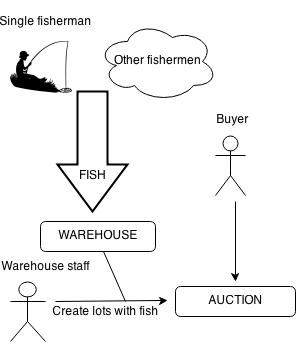
\includegraphics[scale=0.8]{richpic.jpg}
\\
The system must provide means of adding the data about the fish caught by every single fisherman. This will be a website which gives the fisherman the opportunity to enter the amount of fish caught, along with it's type and size. Once this is completed, the fish is taken to the warehouse. According to the data entered by the fishermen, trained staff will  form lots of fish. Those lots will be shown in the website. From there on, every registered buyer will have the chance of participating in the online auctions, and buy the fish he or she is interested in. 
\subsection{System users.}
There are going to be four different types of users supported by the system, namely fishermen, warehouse staff, buyers and system administrator.\\

The fishermen users will use the system from the quayside. They are non technical users, and the user interface should be easy to use, with lots of opportunities to fix errors. 
The warehouse staff is going to use the system to distribute the caught fish into lots. They are going to be trained to use the interface that is to be built. The buyers will access the site when there are auctions going on, from their own devices. The system administrator is responsible for the creation of other user accounts.
\\
\subsection{System functionality.}
The main functionality of the system is shown on the use case diagram below. \\
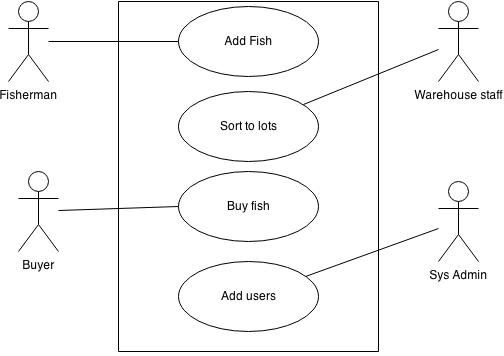
\includegraphics[scale=0.5]{cs223.jpg} \\
The system has the role of identifying any errors and inconsistencies at all times when data is manipulated or added. When the auction for a fish lot finishes, the system has must determine who wins it. Upon that, the appropriate response is given to all the buyers participating in the auction. The auction winner is redirected to another website (not supported by this system) to process the payment details.
\subsection{Data flow analysis.}
The data in the web server will be initially generated from the fishermen. Once the data is entered through the first website, trained staff will use second website to work on the data. Batches with fish will be formed. From there on, the data(batches) can be viewed by the buyers.\\ 
The above data flow diagram shows rough estimate on how the data flows in the system.\\
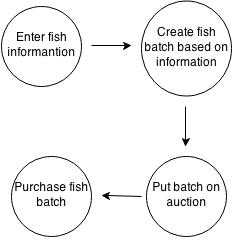
\includegraphics[scale=1]{dataflow.jpg}

\section{Interaction design.}
\subsection{Fishermen's website}
It is crucial that the process of adding fish is correct. Because of that, most emphasis must be put in the design of the interface to be used by the fishermen. It must be extremely friendly, allowing them to correct any mistakes. Their environment is expected to be very busy and distracting, so the website must be flawless, but forgiving in the same time.\\\\
The fisherman page will have only two areas of interest. The first one will be visual representation of all the batches associated with his account. This will be a table showing the data he has entered previously. Each row will represent a single batch. A row will have two buttons associated with. They will be used to print and delete a batch from the table. It is important that we allow the user to remove a batch, if he entered wrong data.\\\\
The second area of interest is going to be a small window, which allows the fisherman to enter a new batch. This will be represented by set of drop down boxes, input fields, and a button "Add". When the user enters the data, and presses the add button, a new table row will appear in the first area of interest, along with notification pop up window. It is important to give the user constant feedback.
\subsection{Warehouse staff's website}
Since the staff is expected to work quickly through on the data, the user interface will provide many shortcuts, and will probably be bloated with many options and configurations. The target auditory is expected to know every detail on the page, that they work on. The interface will be less friendly to novices, and is probably not going to be used by such.\\\\
The staff's website will be a list of batches not currently associated with an auction lot. There will be various means of sorting the list. Even raw SQL statements can be accepted. In the list there will be a check box against each batch. The warehouse worker will select and appropriate set of fish batches, using the check boxes, and create a lot.\\\\ There is a lot of room for errors here, as the worker can potentially create a lot with different fish species in it. He could also mess up with the SQL statements, potentially causing harm to the underlying DBMS.  However, the worker is supposed to know what he is doing at all times, as he will be trained to use the website.
\subsection{Buyers' website}
 The buyers' website will be the one that targets largest auditory. It must be easy to use by both first-time buyers and advanced buyers, who buy fish from the website periodically. This will include search engine so that new users can find the fish they are looking for. Along with that, navigation bars with many categories with different fish types and sizes will be present to allow quick access for the  experienced users. Since the buyers can access the website from any kind of device, a mobile version of the website can also be considered.
\subsection{Admin}
As the requirement specification is not very clear about that, it is possible that the admin will not actually be a user, but rather a underlying function of the system. That is everyone who accesses the main page, can have a "register" option. But for the current prototype the admin user will be provided a page through which he can register the above set of users.

\subsection{Accessibility and customisation}
Each page that is part of the system, should have accessibility options, allowing the user to change the visual representation of the site. Such as the font sizes, color theme and language used.
\section{Prototype}
\url{http://users.aber.ac.uk/enm3/cs22310/login.html}
\section{Evaluation}
\subsection{Consistency}
The visual appearance throughout the set of websites is the same. The active areas all have the background color. All the clickable buttons share the same shape. The predefined choices are in drop down boxes. 
\subsection{Shortcuts}
Shortcuts are provided for the warehouse workers, as they are going to be using the website most frequently. They can use predefined searches as well as direct SQL manipulation of the data. A way to add batches for fisherman could be implemented so that many batches can be added at once. That would of course increase the contents of the page, and it was dropped, as we strive for simplicity when the fisherman is using the website.
\subsection{Feedback}
Feedback is presented to the user by various pop up window boxes. Those should be replaced in the real website with a notification bar, as those windows could get annoying over time. When an action occurs that adds a fish batch(fisherman), creates a lot with fish(worker) or makes a bid(buyer)  an appropriate message is shown to the corresponding user. 
\subsection{Dialog to yield closure}
There wasn't specified requirement for beginning and ending phases in any action supported by the system. Because of that  users' perspective doesn't have any indications showing how close you are to the end.
\subsection{Error handling}
Confirmation is required when batch is to be deleted, so a fisherman can recover from an accidental click. Apart from that, there are no other actions that can cause serious damage. A fact that has to be mentioned here is that the warehouse worker has direct access to the underlying DBMS, and thus is a delicate part of the web server. It is assumed that the warehouse worker is trained, and has other facilities to recover from error.
\subsection{Reversal of actions}
The fishermen can delete any batch they have added with wrong data in it. This should make them not worry even if they don't succeed adding their batch from the first time.
\subsection{Internal locus of control}
There isn't much to be said on this topic. Once the user logs in the system, he is not forced to do any action until he wishes to do so. The system responds appropriately, when and only when the user initiates some action. The user can logout of the system any time.
\subsection{Reduce short-term memory load}
When user logs in the system, he is redirected directly to the page where he has busyness in. No menus, no anything forcing the user to remember where he has to click in order to get to the place where he wants to get. All the text throughout the pages is really brief.




\end{document}